\label{ch:experimental_techniques}

\section{LIBS}
\label{sec:LIBS}
Laser-Induced Breakdown Spectroscopy (LIBS) is an atomic emission spectroscopy technique that utilizes high energy laser pulses to create plasma on the surface of material samples. It is a promising method in analytical chemistry and material analysis because it allows for the direct analysis of solid, liquid and even gas samples, without requiring any chemical preparation.
\\
The interaction between focused laser pulses and the sample leads to the creation of a plasma composed of ionized matter. This plasma emission can yield spectral signatures indicative of the chemical composition of various materials, regardless of their state of matter [Source: Fundamentals and Applications].
\\
LIBS offers the capability of conducting both qualitative and accurate quantitative analyses. Qualitative analysis involves discriminating between different components of a target sample, whereas quantitative analysis goes further by not only identifying the chemical components but also determining their relative concentrations.
\\
However, due to the modest repeatability of the method, attributed to the high variability present between each experiment [Source: Applications of single-shot laser], LIBS doesn’t enable researchers to achieve detection limits and precision as low as those attainable with other methods. Consequently, it is primarily utilized for qualitative, semi-quantitative, or comparative analysis.
\\
The promising performance of this spectroscopy technique as a quantitative chemical analysis system has been facilitated by the development of new spectral processing algorithms in the last decade. These advancements have significantly broadened the application fields of LIBS. Today, LIBS finds applications ranging from diagnostics of archaeological objects to remote material assessment in nuclear power plants, and from the analysis of metal diffusion in solar cells to geological analysis in space explorations.

\subsection{LIBS technique}
\label{subsec:LIBS_technique}
The processes involved in LIBS include laser-sample interaction, material removal, breakdown process, and element-specific emission.
\\
Initially, the interaction between focused laser pulses and the target sample leads to the vaporization of a specific part of the surface area as the temperature reaches the sample material’s boiling point. The evaporated material forms a plume above the sample surface, and due to the continuous energy absorption of the laser, can result in the generation of a high-temperature plasma that will expand and eventually cool down.
[Analytical Chemistry LIBS]

\begin{figure}[H]
    \centering
    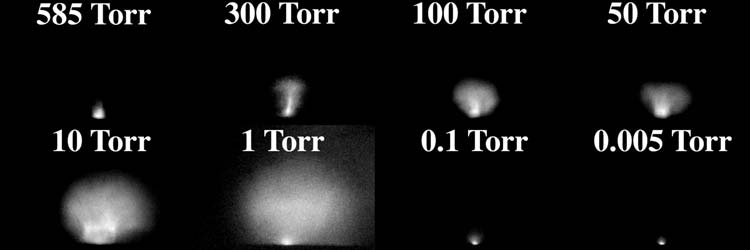
\includegraphics[width = \textwidth]{chapter_1/plasma_expansion_photo.png}
    \label{fig:plasma_expansion}
    \\[20pt]
    \caption[Photo of a plasma expanding.]{Change in visual appearance of the laser plasma formed on soil as the air pressure was reduced.}
\end{figure}
[PHOTO TAKEN FROM LIBS: FUNDAMENTALS AND APPLICATIONS]

The light emitted from the plasma is indicative of the chemical composition of various materials. Positive identification of multiple elemental lines, including both wavelength and intensity within the emission spectrum, contributes to forming a unique spectral fingerprint of the target material. [Fundamentals and applications]
\\
The primary processes that occur during LIBS can be outlined in the following steps:

\begin{enumerate}
\item A short laser pulse is focused on the target material.
\item The incident optical energy is deposited on the sample, resulting in the vaporization of a small amount of its surface.
\item The incoming laser pulse, if its duration is sufficiently large, will also interact with the vapor plume to generate a high-temperature plasma.
\item The system employs a lens or an optical fiber to collect the light emitted from the plasma.
\item A dispersing device, such as a diffraction grating, spatially separates the emitted light into its components. This light originates from the spontaneous emission of hot atoms/ions in the plasma.
\item A digital sensor, such as a CCD or a PMT, is used to collect the light and generate the spectrum.
\item The wavelength and intensity of the resulting atomic emission peaks are analyzed to determine both the chemical elements present in the target sample and their relative concentrations.
\end{enumerate}
Each firing of the laser produces a single LIBS measurement. Typically, however, the signals from many laser plasmas are added or averaged to increase accuracy and precision and to average out non-uniformities in sample composition. [LIBS Cambridge]

\begin{figure}[H]
    \centering
    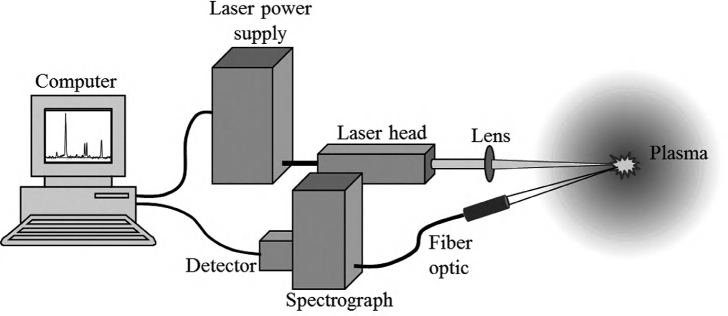
\includegraphics[width = \textwidth]{chapter_1/libs_setup.jpg}
    \label{fig:libs_setup}
    \\[20pt]
    \caption{A schematic of a general apparatus for laser-induced breakdown spectroscopy illustrating the principal components.}
\end{figure}
[PHOTO TAKEN FROM HANDBOOK OF LIBS]

\subsection{Laser-sample Interaction}
\label{subsec:laser-sample_int}

When an atom absorbs a photon, it enters an excited state, where one of its electrons is promoted to a higher energy level. However, the excited states are not very stable, and electrons tend to transition to lower unpopulated energy levels either radiatively, when a photon is generated during the deexcitation process, and non-radiatively when the energy is dissipated in other forms, such as heat or vibration.
\\
Additionally, if the energy applied to the atom is sufficiently high to overcome the ionization potential, electrons can be detached from the atom, creating free negatively charged particles (electrons) and positively charged ions (cations). Initially, the outermost electron, with the lowest ionization potential, is the first to be detached. However, if the supplied energy is high enough, subsequent ionization potentials can be overcome, leading to the detachment of other electrons closer to the nucleus.
\\
There are two main steps leading to breakdown due to optical excitation. The first involves generating a few free electrons that serve as initial receptors of energy through collisions with photons and neutrals. The second is avalanche ionization in the focal region. Free electrons are accelerated by the electric field of the photons, and as the kinetic energy of the electrons grows, collisions will lead to further ionization that will generate even more electrons, creating an avalanche of ionization. 
\\
When a high-energy laser pulse is focused on the surface of a sample, if the irradiance at the focal point exceeds a certain threshold, atoms and ions are ejected from the surface in a process called ablation.

\begin{figure}[H]
    \centering
    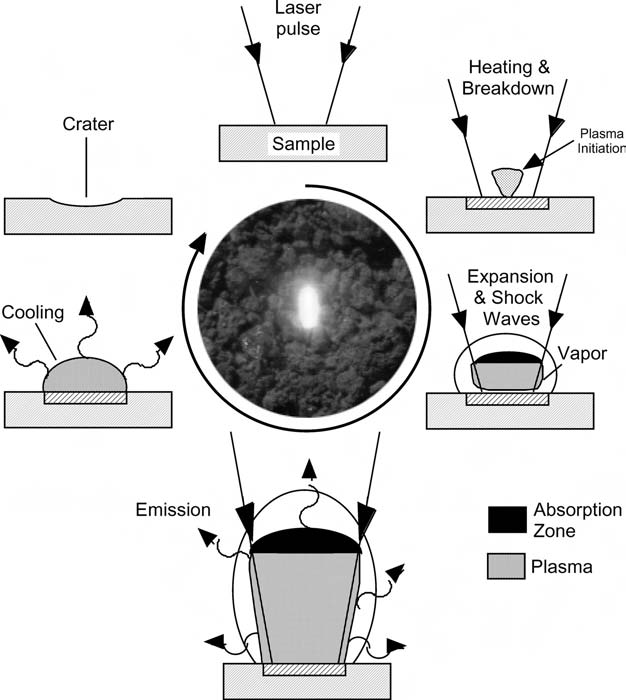
\includegraphics[width = 0.6\textwidth]{chapter_1/libs_life_cycle.png}
    \label{fig:libs_setup}
    \\[40pt]
    \caption[LIBS life cycle.]{Life cycle diagram showing main events in the LIBS process.}
\end{figure}
[PHOTO TAKEN FROM Fundamentals and Applications]

\subsection{Plasma in LIBS}
\label{subsec:plasma_in_libs}
Given the numerous physical and chemical variables characterizing this state, various definitions of plasma are possible. A plasma can be defined as a local assembly of atoms, ions, molecules, and free electrons, that are overall electrically neutral and exhibit a collective behavior.
\\
Under typical conditions, such as atmospheric pressure and temperature, gases are primarily neutral, with only a marginable amount of charged particles. However, at high temperatures ($T > 1000K$), thermal dissociation of atoms and molecules occurs. Plasma forms when the average kinetic energy of the electrons (given by $k_bT$), significantly surpasses the average binding energy of an electron in an ion.
\\
Plasmas are characterized by a variety of parameters, such as the degree of ionization, the plasma temperature, and the electron density. Depending on the degree of ionization a plasma can be categorized as “weakly ionized”, where the ratio between electrons and other species is less than 10\%, or as “highly ionized” where, on the other hand, atoms could be stripped of many electrons, resulting in a very high electrons to ions ratio. LIBS plasmas typically fall in the first category of weakly ionized plasmas; in the figure we can see how LIBS plasmas compare in temperature and electron density relative to other types of plasma.
\begin{figure}[H]
    \centering
    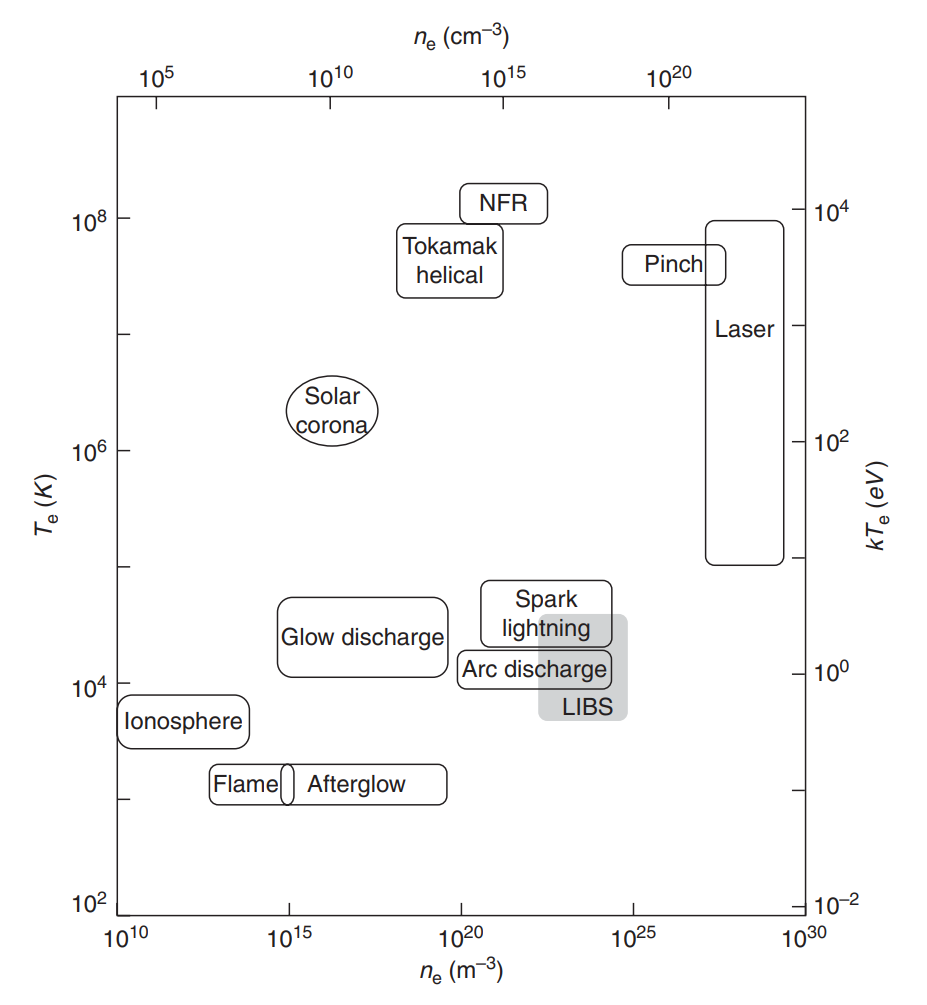
\includegraphics[width = 0.8\textwidth]{chapter_1/plasma_parameters.png}
    \label{fig:plasma_parameters}
    \\[40pt]
    \caption{Relation between plasma parameters and type of plasma.}
\end{figure}
[PHOTO TAKEN FROM HANDBOOK OF LIBS]
The characteristics of the radiation emitted by the plasma depend on the type of radiative transitions that are occurring. At earlier times, where the plasma ionization level is high, the emission will be dominated by a continuum produced by both the bremsstrahlung (free-free transition) and the recombination processes (free-bound transition). Recombination occurs when a free electron is captured by a free ion, releasing its kinetic energy radiatively; while in bremsstrahlung the light is emitted due to electrons being accelerated or decelerated in collisions.
\\
However, the most interesting emissions that can be used for elemental analysis are caused by bound-to-bound transitions that occur between energy levels of ions, atoms, and molecules. 
\begin{figure}[H]
    \centering
    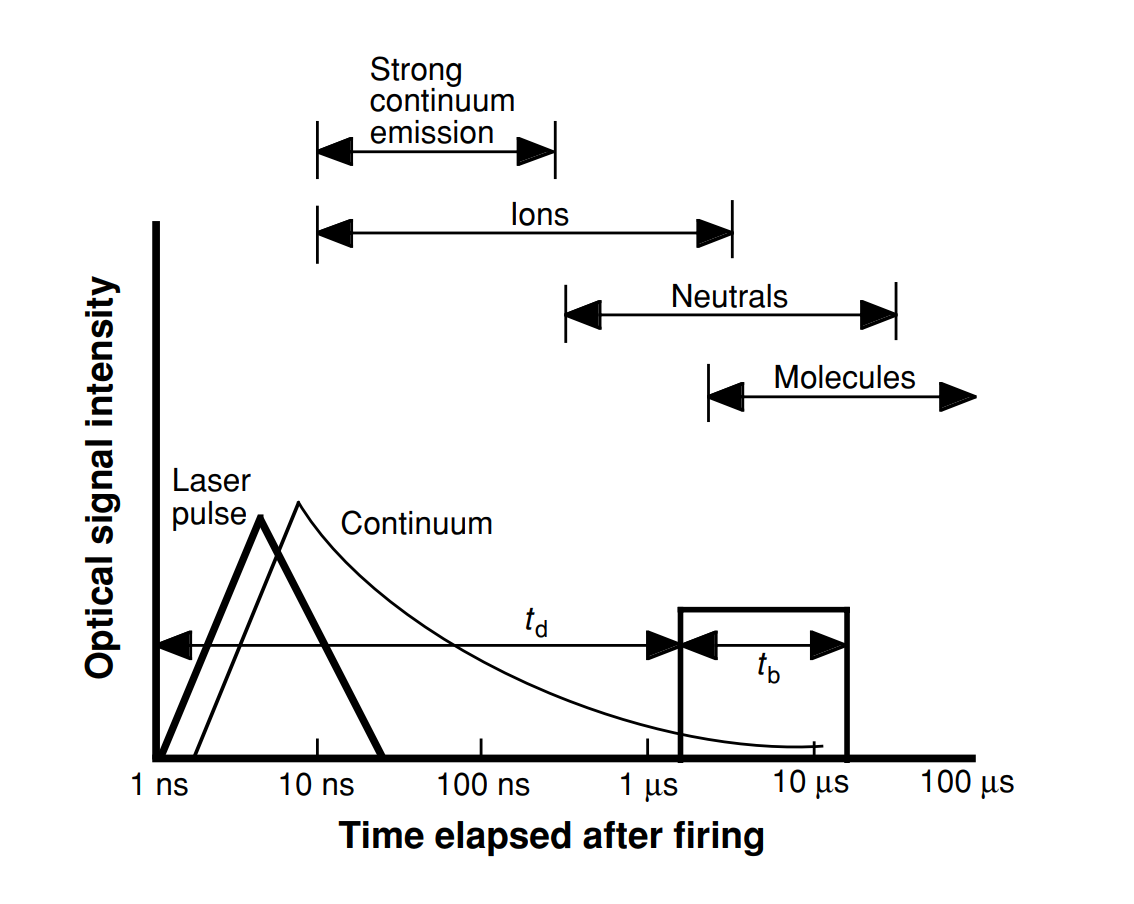
\includegraphics[width = \textwidth]{chapter_1/time_plasma_emission.png}
    \label{fig:time_plasma_emission}
    \\[20pt]
    \caption{Evolution of the emission of the LIBS plasma over time.}
\end{figure}

\subsubsection{Plasma Parameters and Emission Characteristics}
\label{subsubsec:plasma_parameters}
Bound-to-bound transitions are characterized by a fixed energy value, equal to the energy difference between the initial and final level. However, experimentally we see that the measured emission spectrum is not constituted by a collection of sharp lines, but of bell curves instead, with different FWHM. This is because spectral line profiles are also influenced by broadening mechanisms; specifically, pure Doppler broadening, caused by the thermal movement of the emitting particles, will lead to a Gaussian profile, while natural line broadening, due to the time-energy uncertainty principle, and collision broadening will lead to a Lorentzian profile. The collisions between ions and electrons will result in Stark broadening due to the presence of high intensity electric fields near the particles; this phenomenon is predominant in plasmas with higher electron densities, due to the higher probability of collision. 
\\
The Stark broadening causes energy levels to be split according to the value of the quantum number $m_j$, associated with the $z$ component of the total angular momentum $J$, resulting in an asymmetric broadening.
The overall line shape depends on the relative intensity of the different broadening mechanisms and will have a resulting profile obtained by the convolution of the Gaussian and Lorentzian curves, called a Voigt profile.